%%%%%%%%%%%% \todo{FIX LONG COPIED STUFF, and add preliminaries, and add pictures}

\documentclass{beamer}

\usepackage{mathtools}
\newcommand{\defeq}{\vcentcolon=}
\DeclarePairedDelimiter{\paren}{(}{)}

\newcommand{\dec}{\operatorname{dec}}
\newcommand{\poly}{\operatorname{poly}}
\newcommand{\polylog}{\operatorname{polylog}}
\newcommand{\github}{\url{github.com/awestover/Parallel-Partition}}
\newcommand{\defn}[1]       {{\textit{\textbf{\boldmath #1}}}}
\renewcommand{\paragraph}[1]{\vspace{0.09in}\noindent{\bf \boldmath #1.}} 
\usepackage{amsmath}
\def\E{\operatorname{\mathbb{E}}}
\usepackage{amssymb}
\usepackage{amsthm}
\usepackage{todonotes}

\newtheorem{prop}{Proposition}
\newtheorem{cor}{Corollary}
\newtheorem{thm}{Theorem}

\usepackage{hyperref}




\title{Cache-Efficient Parallel Partition}
\author{Alek Westover}
\institute{MIT PRIMES}
\date{2019}

\begin{document}
 
\frame{\titlepage}

\begin{frame}[t]{Introduction}
	\begin{itemize}
		\item What is the partition problem?
		\item Why is it interesting to solve?
	\end{itemize}
	\begin{figure}
		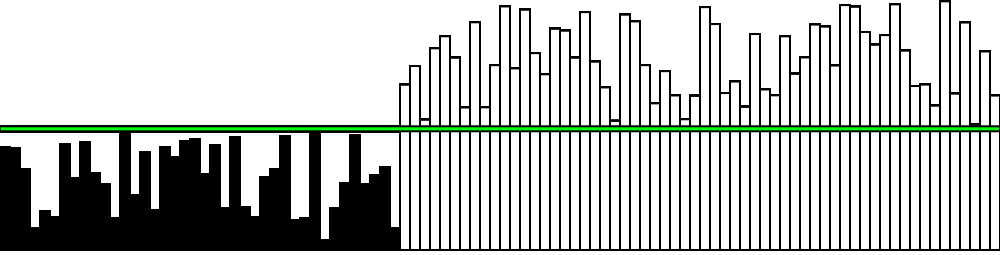
\includegraphics[width=\linewidth]{partitionedArray.png}
		\caption{A depiction of a partitioned array where rectangle heights represent values in the array, and the green bar represents the value the elements are partitioned relative to. Note that the elements colored black are called predecessors and the elements colored white are called successors.}
		\label{fig:partitionedArray}
	\end{figure}
\end{frame}

\begin{frame}[t]{The Partition Problem}
	\begin{itemize}
		\item Given an array $A$ of size $n$ and a decider function that labels each $A[i]$ as either a predecessor or a successor, a partition algorithm must reorder the array such that for all $i$ such that $A[i]$ is a predecessor and for all $j$ such that $A[j]$ is a successor $i < j$.
		\item We will use a decider funciton that partitions the array relative to some "pivot value". That is, we use a decider function that, given some pivot value, labels $A[i]$ a predecessor if and only if $A[i] \le \text{pivot value}$.
\end{itemize}
\end{frame}

\begin{frame}[t]{Parallel Partition Motivation}
	\begin{itemize}
		\item Parrallel partition plays a central role in Parallel Quicksort
		\item Parallel partition is interesting in its own right
		\item Parallel partitions are used in performing filter opperations
\end{itemize}	
\end{frame}

\begin{frame}[t]{Preliminaries}
	\begin{itemize}
		\item Serial Partition
		\item What is parallel processing?
		\item Standard Parallel Partition (not in-place)
		\item Work, Span, and Brent's theorem
		\item With High Probability
		\item Bill's alg and bandwidth bound
		\item Cache Misses
	\end{itemize}
\end{frame}

\begin{frame}[t]{Serial Partition}
\begin{enumerate}
	\item{Initialize \defn{low} to point at the beginning of the array, and initialize \defn{high} to point at the end of the array}
	\item{Increment low until $A[\text{low}]$ is a successor}
	\item{Decrement high until $A[\text{high}]$ is a predecessor}
	\item{Swap values $A[\text{low}]$ and $A[\text{high}]$ in the array}
	\item{Repeat steps 3-5 until $\text{high} \geq \text{low}$ which means that all elements in the array have been processed}
	\item{If $A[\text{low}]$ is a predecessor increment $A[\text{low}]$ by $1$ so that $A[\text{low}]$ is the first successor in $A$, which is now partitioned}
\end{enumerate}
This has work $O(n)$, is in-place, and incurs $n+O(1)$ cache misses.	
\end{frame}

\begin{frame}[t]{Standard Parallel Partition (not in-place)}
	\begin{itemize}
		\item Parallel prefix sum
	\end{itemize}
\end{frame}

\begin{frame}[t]{Work, Span, Brent's Theorem}
	\begin{itemize}
		\item The \defn{work} of an algorithm, denoted $T_1$	is its running time with a single processor.
		\item The \defn{span} of an algorithm, denoted $T_\infty$ is its running time with an infinite number of processors.
		\item Clearly $T_p \ge \frac{T_1}{p}$ and $T_p \ge T_\infty$.
		\item Brent's theorem gives an upper bound for an algorithm's running time on $p$ processors, denoted $T_p$, from the alghrithms work and span. 
	\end{itemize}
	\begin{thm}[Brent's theorem]
		$$ T_p \le \frac{T_1}{p} +  T_\infty.$$
	\end{thm}
\end{frame}

\begin{frame}[t]{With High Probability}
	whp means $$1-n^{-c}$$
	for $c$ of our choice.
\end{frame}

\begin{frame}[t]{Bill's alg and Memory Bandwidth Bound}
	Memory bandwidth bound is bad. Thus minimizing cache misses is good.
	
\end{frame}

\begin{frame}[t]{Cache Misses}
	defn
\end{frame}

\begin{frame}[t]{The Strided Algorithm}
	\begin{itemize}
		\item Description
		\item Guarantees
\end{itemize}	
\end{frame}

\begin{frame}[t]{Description}
\begin{itemize}
\item \textbf{The Partial Partition Step.} Let $g \in \mathbb{N}$ be a
  parameter, and assume for simplicity that $gb \mid n$. Partition the
  array $A$ into $\frac{n}{gb}$ chunks $C_1, \ldots, C_{n / gb}$,
  each consisting of $g$ cache lines of size $b$.
	For $i \in \{1, 2, \ldots, g\}$, define 
  $P_i$ to consist of the $i$-th cache line from each of the
  chunks $C_1, \ldots, C_{n / gb}$. One can think of the $P_i$'s
	as forming a strided partition of array $A$, since
  consecutive cache lines in $P_i$ are always separated by a fixed
  stride of $g - 1$ other cache lines.

  The first step of the algorithm is to perform an in-place serial
  partition on each of the $P_i$s, rearranging the elements within the
  $P_i$ so that the predecessors come first. %This step requires work $\Theta(n)$ and span $\Theta(n/g)$.
\item \textbf{The Serial Cleanup Step. }For each $P_i$, define the \defn{splitting position} $v_i$ to be
  the position in $A$ of the final predecessor in (the already
  partitioned) $P_i$. Define $v_{\text{min}} = \min\{v_1, \ldots,
  v_{g}\}$ and define $v_{\text{max}} = \max\{v_1, \ldots, v_{g}\}$. Then the
  second step of the algorithm is to perform a serial partition on the
	sub-array \\$A[v_{\text{min}}],\ldots, A[v_{\text{max}}-1]$. This completes the   
    full partition.
\end{itemize}

\end{frame}

\begin{frame}[t]{Guarantees}
	Note that the partial partition step has parallelism, and requires work $\Theta(n)$ and span $\Theta(n/g)$.
Note that the Cleanup Step of the Strided Algorithm has no
parallelism, and thus has span $\Theta(v_{\text{max}} -
v_{\text{min}})$.  In general, this results in an algorithm with
linear-span (i.e., no parallelism guarantee).  When the number of
predecessors in each of the $P_i$'s is close to equal, however, the
quantity $v_{\text{max}} - v_{\text{min}}$ can be much smaller than
$O(n)$.  For example, if $b = 1$, and if each element of $A$ is
selected independently from some distribution, then one can use
Chernoff bounds to prove that with high probability in $n$,
$v_{\text{max}} - v_{\text{min}} \le O(\sqrt{n \cdot g \cdot \log
  n})$.  The full span of the algorithm is then $\tilde{O}(n/g +
\sqrt{n \cdot g})$, which optimizes at $g = n^{1/3}$ to
$\tilde{O}(n^{2/3})$. Since the Partial Partition Step incurs only $n
/ b$ cache misses, the full algorithm incurs $n + \tilde{O}(n^{2/3})$ cache
misses on a random array $A$.


Using Hoeffding's Inequality in place of Chernoff bounds, one can
obtain analogous bounds for larger values of $b$; in particular for $b
\in \operatorname{polylog}(n)$, the optimal span remains
$\tilde{O}(n^{2/3})$ and the number of cache misses becomes $n / b +
\tilde{O}(n^{2/3} / b)$ on an array $A$ consisting of randomly sampled
elements.\footnote{The original algorithm of Francis and Pannan
  \cite{FrancisPa92} does not consider the cache-line size $b$. Frias
  and Petit later introduced the parameter $b$ \cite{Frias08}, and
  showed that by setting $b$ appropriately, one obtains an algorithm
  whose empirical performance is close to the state-of-the-art.}
\end{frame}

\begin{frame}[t]{The Smoothed Striding Algorithm}
	\begin{itemize}
		\item Partial Partition Description
		\item Partial Partition Analysis 
		\item From Partial Partition to Full Partition
		\item Hybrid Smoothed Striding Algorithm
		\begin{itemize}
			\item Theorem
			\item Corollary
		\end{itemize}
		\item Recursive Smoothed Striding Algorithm
		\begin{itemize}
			\item Theorem
			\item Corollary
		\end{itemize}
	\end{itemize}
\end{frame}

\begin{frame}[t]{Partial Partition Description}
	\begin{itemize}
\item Set each of $X[1], \ldots, X[s]$ to be uniformly random and
  independently selected elements of $\{1, 2, \ldots, g\}$. For
  $i \in \{1, 2, \ldots, g\}$, and for each $j \in \{1, 2,
  \ldots, s\}$, define
  $$G_i(j) = (X[j] + i \pmod g) + (j - 1)g + 1.$$ Using this
  terminology, we define each $U_i$ for $i \in \{1, \ldots, g\}$ to
  contain the $G_i(j)$-th cache line of $A$ for each $j \in \{1, 2,
  \ldots, s\}$. That is, $G_i(j)$ denotes the index of the $j$-th
  cache line from array $A$ to be contained in $U_i$.

  Note that, to compute the index of the $j$-th cache line in $U_i$,
  one needs only the value of $X[j]$. Thus the only metadata needed by
  the algorithm to determine the $U_1, \ldots, U_g$ is the array
  $X$. If $|X| = s = \frac{n}{gb} \le \operatorname{polylog}(n)$, then
  the algorithm is in place.
  
\item The algorithm performs an in-place (serial) partition on each
  $U_i$ (and performs these partitions in parallel with one
  another). In doing so, the algorithm, also collects
  $v_{\text{min}}=\min_i{v_i}$, $v_{\text{max}}=\max_i{v_i}$, where
	each $v_i$ with $i \in \{1, \ldots, g\}$ is defined to be the index
  of the final predecessor in $A$ (or $0$ if no such predecessor
  exists).\footnote{One can calculate $v_{\text{min}}$ and
    $v_{\text{max}}$ without explicitly storing each of $v_1, \ldots,
		v_{g}$ as follows. Rather than using a standard $g$-way parallel
		for-loop to partition each of $U_1, \ldots, U_{g}$, one can
    manually implement the parallel for-loop using a recursive
    divide-and-conquer approach. Each recursive call in the
    divide-and-conquer can then simply collect the maximum and minimum
    $v_i$ for the $U_i$'s that are partitioned within that recursive
    call. This adds $O(\log n)$ to the total span of the Partial
    Partition Step, which is does not affect the overall span
    asymptotically. %% In practice, this can also be implemented using
    %% CilkPlus Reducers (or OpenMP Reductions) \cite{FrigoLe09}, though
    %% empirically we have found explicitly implementing the
    %% divide-and-conquer structure to be worthwhile for performance.
  }
  
  The array $A$ is now partially partitioned, i.e. $A[i]$ is a
  predecessor for all $i \le v_{\text{min}}$, and $A[i]$ is a successor
  for all $i > v_{\text{max}}$.
\end{itemize}

\end{frame}

\begin{frame}[t]{Partial Partition Step Analysis}
\begin{proposition}
  \label{prop:generalResult}
  %% The 1/2's are necessary for the final line of the proof to easily go through.
  
  Let $\epsilon \in (0, 1/2)$ and $\delta \in (0, 1/2)$ such that
  $\epsilon \ge \frac{1}{\poly(n)}$ and $\delta \ge
  \frac{1}{\polylog(n)}$. Suppose $s > \frac{\ln
    (n/\epsilon)}{\delta^2}$. Finally, suppose that each processor has
  a cache of size at least $s + c$ for a sufficiently large constant
  $c$.

  Then the Partial-Partition Algorithm achieves work $O(n)$; achieves
  span $O\paren*{b \cdot s}$; incurs $\frac{s+n}{b} + O(1)$ cache
  misses; and guarantees with probability $1 - \epsilon$ that
  $$v_{\text{max}}-v_{\text{min}} < 4 n \delta.$$
\end{proposition}
\end{frame}

\begin{frame}[t]{From Partial Partition to Full Partition}
We will use Proposition \ref{prop:generalResult} as a tool to analyze the Recursive and the Hybrid Smoothed Striding Algorithms.

Rather than parameterizing the Partial Partition step in each algorithm by $s$, Proposition \ref{prop:generalResult} suggests that it is more natural to parameterize by $\epsilon$ and $\delta$, which then determine $s$.

We will assume that both the hybrid and the recursive algorithms use $\epsilon = 1/n^c$ for $c$ of our choice (i.e. with high probability in $n$). Moreover, the Recursive Smoothed Striding Algorithm continues to use the same value of $\epsilon$ within recursive subproblems (i.e., the $\epsilon$ is chosen based on the size of the first subproblem in the recursion), that way the entire algorithm succeeds with high probability in $n$.

For both algorithms, the choice of $\delta$ results in a tradeoff between cache misses and span. For the Recursive algorithm, we allow for $\delta$ to be chosen arbitrarily at the top level of recursion, and then fix $\delta  = \Theta(1)$ to be a sufficiently small constant at all levels of recursion after the first; this guarantees that we at least halve the size of the problem size between recursive iterations\footnote{In general, setting $\delta = 1/8$ will result in the problem size being halved. However, this relies on the assumption that $gb \mid n$, which is only without loss of generality by allowing for the size of subproblems to be sometimes artificially increased by a small amount (i.e., a factor of $1 + gb / n = 1 + 1/s$). One can handle this issue by decreasing $\delta$ to, say, $1/16$.}. Optimizing $\delta$ further (after the first level of recursion) would only affect the number of undesired cache misses by a constant factor.
\end{frame}

\begin{frame}[t]{Hybrid Algorithm Analysis - General Theorem}
\begin{theorem}
	\label{thm:fullPartition}
	The Hybrid Smoothed Striding Algorithm algorithm using parameter $\delta\in(0,1/2)$ satisfying $\delta \ge 1/\polylog(n)$: has work $O(n)$; achieves span
        $$O\paren*{\log n \log\log n +\frac{b\log n}{\delta^2}},$$
with high probability in $n$; and incurs fewer than 
$$(n+O(n\delta))/b$$
cache misses with high probability in $n$.
\end{theorem}
\end{frame}

\begin{frame}[t]{Hybrid Algorithm Analysis - Corollary for specific parameter settins}
An interesting corollary of the above theorem concerns what happens when $b$ is small (e.g., constant) and we choose $\delta$ to optimize span. 
\begin{corollary}[Corollary of Theorem \ref{thm:fullPartition}]
	\label{cor:fullPartition}
Suppose $b \le o(\log \log n)$. Then the Cache-Efficient Full-Partition Algorithm algorithm using $\delta = \Theta\big(\sqrt{b/\log\log n}\big)$, achieves work $O(n)$, and with high probability in $n$, achieves span $O(\log n \log\log n)$ and incurs fewer than $(n+o(n))/b$ cache misses.\\\\
\end{corollary}
\end{frame}


\begin{frame}[t]{Recursive Algorithm Analysis - General Theorem}
	\begin{theorem}
	\label{thm:groupedPartitionAlg}
	With high probability in $n$, the Recursive Smoothed Striding
        algorithm using parameter $\delta \in(0,1/2)$ satisfying
        $\delta \ge 1 / \polylog(n)$: achieves work $O(n)$, attains span
	$$O\left(b\left(\log^2 n + \frac{\log n}{\delta^2}\right)\right),$$
	and incurs $(n+O(n \delta))/b$ cache misses. 
\end{theorem}
\end{frame}

\begin{frame}[t]{Recursive Algorithm Analysis - Corollary for specific parameter settings}
A particularly natural parameter setting for the Recursive algorithm occurs at $\delta = 1 / \sqrt{\log n}$.
\begin{corollary}[Corollary of Theorem \ref{thm:groupedPartitionAlg}]
  \label{cor:groupedPartitionAlg}
	With high probability in $n$, the Recursive Smoothed Striding Algorithm using parameter $\delta=1/\sqrt{\log n}$:
  achieves work $O(n)$, attains span $O(b\log^2 n)$, and incurs $n/b \cdot (1 + O(1 / \sqrt{\log n}))$ cache misses. 
\end{corollary}
\end{frame}

\begin{frame}[t]{Expiriments}
	\begin{itemize}
		\item Strided Algorithm vs Smoothed Striding algorithm
		\item Cache misses 
	\end{itemize}
\end{frame}

\begin{frame}[t]
\frametitle{Acknowledgments}
I would like to thank
\begin{itemize}
	\item {The MIT PRIMES program}
	\item {William Kuszmaul, my PRIMES mentor}
	\item {My parents}
\end{itemize}
\end{frame}

\end{document}
